\chapter{Specifikacija programske potpore}
		
	\section{Funkcionalni zahtjevi}
		\noindent \textbf{Dionici:}
		
    		\begin{packed_enum}
    			\item Naručitelj
    			\item Javnost
    			\item Korisnici
    			\item Organizator
    			\item Glazbenik 	
    			\item Voditelj benda						
    			\item Administrator
    			\item Razvojni tim
    		\end{packed_enum}
		
		\noindent \textbf{Aktori i njihovi funkcionalni zahtjevi:}
		
		
		\begin{packed_enum}

		\item  \underbar{Neprijavljeni/neregistrirani korisnik (javnost) može:}
						
			\begin{packed_enum}
				\item Pregledati javne događaje
				\item Pregledati profil benda
				\item Pročitati recenzije
				\item Registrirati se na aplikaciji
			\end{packed_enum}
					
		\item  \underbar{Korisnik (inicijator) može:}
			
			\begin{packed_enum}
				
				\item Sve što i Javnost
				\item Prijaviti se na aplikaciju
				\item Pregledavati i uređivati korisnički profil
				\item Pregledati postojeće poruke s drugim korisnicima
				\item Pregledati svoj kalendar
				\item Slati nove poruke drugim korisnicima
				\item Recenzirati događaje
				\item Komentirati objave glazbenika
				\item Postati glazbenik i/ili organizator
				\item Pisati objave na svom profilu
				\item Odjaviti se 
				
			\end{packed_enum}
			
			
		\item  \underbar{Glazbenik (inicijator) može:}
			
			\begin{packed_enum}
				
				\item Sve što i Korisnik
				\item Prihvatiti ili odbiti poziv u bend
				\item Postati članom jednog ili više bendova
				\item Održati samostalan nastup
				\item Stvoriti bend
			\end{packed_enum}
			
		\item  \underbar{Organizator (inicijator) može:}
			
			\begin{packed_enum}
				
				\item Sve što i Korisnik
				\item Pretraživati bendove na aplikaciji
				\item Stvarati događaje
				\item Uređivati događaje
				\item Recenzirati bend kao organizator događaja
			\end{packed_enum}
			
		\item  \underbar{Voditelj benda (inicijator) može:}
			
			\begin{packed_enum}
				
				\item Sve što i Glazbenik
				\item Pozivati i dodavati nove članove u bend
				\item Dodavati obaveze u kalendar benda
				\item Vidjeti kalendare članova benda
				\item Recenzirati organizatora u ime benda
				\item Napisati objave na stranici benda
				\item Uređivati profil benda
			\end{packed_enum}
			
		\item  \underbar{Administrator (inicijator) može:}
			
			\begin{packed_enum}
				
				\item Blokirati korisnike koji su prekršili uvjete korištenja aplikacije
				\item Uređivati popis instrumenata
				\item Dodati događaje koji su stvoreni na drugim platformama
				
			\end{packed_enum}
			
		\item  \underbar{Baza podataka (sudionik) može:}
			
			\begin{packed_enum}
				
				\item Pohraniti podatke o korisnicima, glazbenicima, organizatorima i bendovima
				\item Pohraniti podatke o nastupima, recenzijama, objavama, komentarima
				\item Pohraniti razmijenjene poruke između korisnika 
				
			\end{packed_enum}
		
		\end{packed_enum}
			
\eject 
			
			
				
\subsection{Obrasci uporabe}
\subsubsection{Opis obrazaca uporabe}
\noindent \underbar{\textbf{UC1 - Pristup listi javnih događaja}}
	\begin{packed_item}
		
		\item \textbf{Glavni sudionik: } Javnost
		\item  \textbf{Cilj:} Vidjeti listu javnih događaja na aplikaciji
		\item  \textbf{Sudionici:} Baza podataka
		\item  \textbf{Preduvjet:} -
		\item  \textbf{Prioritet:} High
		\item  \textbf{Opis osnovnog tijeka:}
		
		\item[] \begin{packed_enum}
			\item Javnost na početnoj stranici odabire prikaz događaja
			\item Aplikacija prikazuje javne događaje
		\end{packed_enum}
		
	\end{packed_item}


\noindent \underbar{\textbf{UC2 - Pregled profila benda}}
	\begin{packed_item}
	
		\item \textbf{Glavni sudionik:} Javnost
		\item  \textbf{Cilj:} Vidjeti profil benda
		\item  \textbf{Sudionici:} Baza podataka
		\item  \textbf{Preduvjet:} -
		\item  \textbf{Prioritet:} High
		\item  \textbf{Opis osnovnog tijeka:}
		
		\item[] \begin{packed_enum}
			\item Javnost odabire bend čiji profil želi pregledati
			\item Aplikacija prikazuje profil odabranog benda
		\end{packed_enum}
	\end{packed_item}

\noindent \underbar{\textbf{UC3 - Pregled recenzija}}
	\begin{packed_item}
	
		\item \textbf{Glavni sudionik: }Javnost
		\item  \textbf{Cilj:} Vidjeti pregled recenzija
		\item  \textbf{Sudionici:} Baza podataka
		\item  \textbf{Preduvjet:} -
		\item  \textbf{Prioritet:} Medium
		\item  \textbf{Opis osnovnog tijeka:}
		
		\item[] \begin{packed_enum}
			\item Javnost odabire popis recenzija
			\item Aplikacija prikaže popis recenzija
			\item Javnost odabere recenziju koju želi vidjeti
			\item Aplikacija korisniku prikaže odabranu recenziju
		\end{packed_enum}
	\end{packed_item}

	
	\noindent \underbar{\textbf{UC4 - Registracija}}
	\begin{packed_item}
	
		\item \textbf{Glavni sudionik: }Javnost
		\item  \textbf{Cilj:} Registrirati se
		\item  \textbf{Sudionici:} Baza podataka
		\item  \textbf{Preduvjet:} -
		\item  \textbf{Prioritet:} High
		\item  \textbf{Opis osnovnog tijeka:}
		
		\item[] \begin{packed_enum}

			\item Javnost odabire opciju za registraciju
			\item Aplikacija prikazuje prozor za unos podataka
			\item Javnost unosi tražene korisničke podatke
			\item Aplikacija korisniku šalje email za verifikaciju email-a
			\item Korisnik prima obavijest o uspješnoj registraciji
		\end{packed_enum}
		
		\item  \textbf{Opis mogućih odstupanja:}
		
		\item[] \begin{packed_item}

			\item[2.a] Odabir već zauzetog korisničkog imena i/ili e-maila, unos podataka u nedozvoljenom formatu
			\item[] \begin{packed_enum}

				\item Sustav obavještava korisnika o neuspjelom upisu i vraća ga na stranicu za registraciju.
				\item Korisnik mijenja potrebne podatke ili odustaje od registracije.

			\end{packed_enum}
		\end{packed_item}						
	\end{packed_item}

\noindent \underbar{\textbf{UC5 - Prijava u sustav}}
	\begin{packed_item}
	
		\item \textbf{Glavni sudionik: } Korisnik
		\item  \textbf{Cilj:} Korištenje aplikacije
		\item  \textbf{Sudionici:} Baza podataka
		\item  \textbf{Preduvjet:} Napravljena registracija
		\item  \textbf{Prioritet:} High
		\item  \textbf{Opis osnovnog tijeka:}
		
		\item[] \begin{packed_enum}
			
			\item Korisnik odabire opciju "Prijava"
			\item Aplikacija prikazuje prozor za prijavu
			\item Korisnik unosi podatke
			\item Baza autorizira unesene podatke te dozvoljava korisniku korištenje aplikacije
			\item Aplikacija korisniku prikazuje početnu stranicu
		\end{packed_enum}
	
			\item  \textbf{Opis mogućih odstupanja:}
			\item[] \begin{packed_enum}
												
				\item[2.a] Aplikacija ne dozvoljava Korisniku korištenje aplikacije ako su podaci neispravni
				
			\end{packed_enum}
	\end{packed_item}


\noindent \underbar{\textbf{UC6 - Uvid u popis dodanih instrumenata}}
	\begin{packed_item}

		\item \textbf{Glavni sudionik:} Administrator
		\item \textbf{Cilj:} Izmjena krivo unesenih instrumenata u bazi
		\item \textbf{Sudionici:} Baza podataka
		\item \textbf{Preduvjet:} Administrator je prijavljen u sustav
		\item \textbf{Prioritet:} Low
		\item \textbf{Opis osnovnog tijeka:}
		
		\item[] \begin{packed_enum}

			\item Administrator odabire pregled dodanih instrumenata
			\item Baza ispisuje dodane instrumente
			\item Administrator mijena krivo unesene zapise 
		\end{packed_enum}
	\end{packed_item}
			
\noindent \underbar{\textbf{UC7 - Blokiranje korisnika koji su prekršili uvjete korištenja}}
	\begin{packed_item}
		
		\item \textbf{Glavni sudionik: }Administrator
		\item \textbf{Cilj:} Blokirati korisnike koji krše uvjete korištenja aplikacije
		\item \textbf{Sudionici:} Baza podataka
		\item \textbf{Preduvjet:} Administrator je prijavljen u sustav
		\item \textbf{Prioritet:} Low
		\item \textbf{Opis osnovnog tijeka:}
		
		\item[] \begin{packed_enum}
			
			\item Administrator uočava korisnika koji krši opća pravila korištenja sustava
			\item Administrator blokira korisnički račun određenoga korisnika na neodređeno vrijeme
		\end{packed_enum}
	\end{packed_item}

\noindent \underbar{\textbf{UC8 - Dodavanje događaja}}
	\begin{packed_item}
		
		\item \textbf{Glavni sudionik: }Administrator
		\item \textbf{Cilj:} Dodati događaje koji su kreirani van sustava u sustav
		\item \textbf{Sudionici:} Baza podataka
		\item \textbf{Preduvjet:} Administrator je prijavljen u sustav
		\item \textbf{Prioritet:} Low
		\item \textbf{Opis osnovnog tijeka:}
		
		\item[] \begin{packed_enum}
			
			\item Administrator odabire opciju za dodavanje događaja u sustav
			\item Administrator dodaje događaj u sustav
		\end{packed_enum}
	\end{packed_item}

\noindent \underbar{\textbf{UC9 - Pregled poruka}}
	\begin{packed_item}

		\item \textbf{Glavni sudionik: }Korisnik
		\item \textbf{Cilj:} Uvid u postojeće poruke
		\item \textbf{Sudionici:} Baza podataka
		\item \textbf{Preduvjet:} Korisnik je prijavljen
		\item \textbf{Prioritet:} High
		\item \textbf{Opis osnovnog tijeka:}
		
		\item[] \begin{packed_enum}

			\item Korisnik odabire "Poruke"
			\item Aplikacija prikazuje osobe s kojima se već vodio razgovor
			\item Korisnik odabire osobu te se prikazuju poruke
		\end{packed_enum}
	
		\item  \textbf{Opis mogućih odstupanja:}
	
		\item[] \begin{packed_item}

			\item[2.a] Korisnik nema prošlih poruka
			\item[] \begin{packed_enum}
				\item Aplikacija prikazuje poruku „Nema poruka“
			\end{packed_enum}
		\end{packed_item}
	\end{packed_item}

\noindent \underbar{\textbf{UC10 - Pisanje poruke}}
	\begin{packed_item}
		
		\item \textbf{Glavni sudionik: }Korisnik
		\item \textbf{Cilj:} Komunikacija među korisnicima
		\item \textbf{Sudionici:} Baza podataka
		\item \textbf{Preduvjet:} Korisnik je prijavljen
		\item \textbf{Prioritet:} High
		\item \textbf{Opis osnovnog tijeka:}
		
		\item[] \begin{packed_enum}
			
			\item Korisnik odabire poruke
			\item Aplikacija prikazuje korisnikove razgovore
			\item Korisnik odabire drugog korisnika s kojim želi komunicirati
			\item Aplikacija prikazuje postojeće poruke s odabranom osobom
			\item Korisnik unosi novu poruku
			\item Korisnik odabere „Pošalji“ za slanje poruke
		\end{packed_enum}
		
		\item \textbf{Opis mogućih odstupanja:}
		
		\item[] \begin{packed_item}
			
			\item[3.a] Korisnik želi poslati poruku osobi s kojom još nije komunicirao
			\item[] \begin{packed_enum}
				\item Korisnik odabire opciju „Nova poruka“
				\item Pronalazi korisnika kojemu želi napisati poruku
			\end{packed_enum}
		\end{packed_item}
	\end{packed_item}
			
\noindent \underbar{\textbf{UC11 - Pisanje recenzije o bendu}}
	\begin{packed_item}
		
		\item \textbf{Glavni sudionik:} Korisnik
		\item \textbf{Cilj:} Napisati recenziju o bendu
		\item \textbf{Sudionici:} Baza podataka
		\item \textbf{Preduvjet:} Korisnik mora biti prijavljen
		\item \textbf{Prioritet:} Medium
		\item \textbf{Opis osnovnog tijeka:} 
		
		\item[] \begin{packed_enum}
			
			\item Korisnik pristupa profilu benda
			\item Korisnik u okvir za recenzije napiše svoje mišljenje te da ocjenu
			\item Korisnik odabere "Završi recenziju"
		\end{packed_enum}
	\end{packed_item}
				
\noindent \underbar{\textbf{UC12 - Pisanje recenzije za događaj}}
	\begin{packed_item}
		
		\item \textbf{Glavni sudionik:} Korisnik
		\item \textbf{Cilj:} Napisati recenziju za događaj
		\item \textbf{Sudionici:} Baza podataka
		\item \textbf{Preduvjet:} Korisnik je prijavljen
		\item \textbf{Prioritet:} Medium
		\item \textbf{Opis osnovnog tijeka:} 
		
		\item[] \begin{packed_enum}
			
			\item Korisnik odabire opciju za recenziranje događaja
			\item Aplikacija otvara prozor za unos recenzije
			\item Korisnik u okvir za recenzije napiše svoje mišljenje te da ocjenu
			\item Korisnik odabere "Završi recenziju"
			\item Aplikacija sprema recenziju
		\end{packed_enum}
	\end{packed_item}
		 
\noindent \underbar{\textbf{UC13 - Pregled profila korisnika}}
	\begin{packed_item}
	    	
    	\item \textbf{Glavni sudionik: }Korisnik
    	\item \textbf{Cilj:} Pregled profilne stranice korisnika
    	\item \textbf{Sudionici:} Baza podataka
    	\item \textbf{Preduvjet:} Korisnik je prijavljen
    	\item \textbf{Prioritet:} High
    	\item \textbf{Opis osnovnog tijeka:} 
    	
    	\item[] \begin{packed_enum}

    		\item Korisnik odabire prikaz profila korisnika
    		\item Aplikacija prikazuje profil korisnika
    		\item[] \begin{packed_enum}

    			\item Ako je glazbenik onda mu se prikazuju dodatne informacije (kalendar, instrumenti, popis događaja na kojima svira)
    			\item Ako je organizator onda mu se prikazuju dodatne informacije (menager name i recenzije kao organizator)
    		\end{packed_enum}
    	\end{packed_enum}
	\end{packed_item}
	    
\noindent \underbar{\textbf{UC14 - Komentiranje objava glazbenika}}
   	\begin{packed_item}
   		
   		\item \textbf{Glavni sudionik:} Korisnik
   		\item  \textbf{Cilj:} Komentiranje objave glazbenika
   		\item  \textbf{Sudionici:} Baza podataka
   		\item  \textbf{Preduvjet:} Korisnik je prijavljen
   		\item  \textbf{Prioritet:} Medium
   		\item  \textbf{Opis osnovnog tijeka:} 
   		
   		\item[] \begin{packed_enum}
   			\item Korisnik odabire "Komentiraj" na objavi glazbenika
   			\item Aplikacija otvara prozor za unos komentara
   			\item Korisnik piše komentar
   			\item Korisnik odabere "Spremi"
   			\item Aplikacija sprema objavu
   		\end{packed_enum}
   	\end{packed_item}
    	
\noindent \underbar{\textbf{UC15 - Uređivanje profila korisnika}}
	\begin{packed_item}
	
		\item \textbf{Glavni sudionik:} Korisnik 
		\item  \textbf{Cilj:} Promjeniti informacije na profilu
		\item  \textbf{Sudionici:} Baza podataka
		\item  \textbf{Preduvjet:} Korisnik je prijavljen u sustav
		\item  \textbf{Prioritet:} High
		\item  \textbf{Opis osnovnog tijeka:}
		
		\item[] \begin{packed_enum}
			
			\item Korisnik odabire opciju za uređivanje profila 
			\item Korisnik mijenja podatke
			\item Korisnik odabirom opcije za spremanje potvrđuje i sprema načinjene promjene
		\end{packed_enum}
		\item  \textbf{Opis mogućih odstupanja:}
			
			\item[] \begin{packed_item}
				
				\item[3.a] Korisnik nije unio obavezne podatke ili su podatci nevaljani
				\item[] \begin{packed_enum}
					
					\item Korisnik ponovno unosi obavezne podatke
					\item Korisnik odustaje od uređivanja profila
					
				\end{packed_enum}		
			\end{packed_item}
	\end{packed_item}
    	
\noindent \underbar{\textbf{UC16 - Stvaranje profila organizatora}}
   	\begin{packed_item}
   		
   		\item \textbf{Glavni sudionik: }Korisnik
   		\item \textbf{Cilj:} Dodavanje privilegija organizatora korisniku
   		\item \textbf{Sudionici:} Baza podataka
   		\item \textbf{Preduvjet:} Korisnik je prijavljen u sustav
   		\item \textbf{Prioritet:} High
   		\item \textbf{Opis osnovnog tijeka:}
   		
   		\item[] \begin{packed_enum}
   			
   			\item Korisnik odabire uređivanje profila
   			\item Korisnik odabire opciju "Organizator"
   			\item Aplikacija prikazuje dodatna polja za unos informacija
   			\item Korisnik popunjava potrebne informacije
   			\item Korisnik spremanjem promjena postaje Organizator
   			
   		\end{packed_enum}
   		
   		\item  \textbf{Opis mogućih odstupanja:}
   		
   		\item[] \begin{packed_item}
   			
   			\item[5.a] Korisnik nije unio obavezne podatke ili su podatci nevaljani
   			\item[] \begin{packed_enum}
   				
   				\item Korisnik ponovno unosi obavezne podatke
   				\item Korisnik odustaje od izmjene profila
   				
   			\end{packed_enum}
   		\end{packed_item}
   	\end{packed_item}



\noindent \underbar{\textbf{UC17 - Stvaranje profila glazbenika}}
	\begin{packed_item}
		
		\item \textbf{Glavni sudionik: } Korisnik
		\item \textbf{Cilj:} Dodavanje privilegija glazbenika korisniku
		\item \textbf{Sudionici:} Baza podataka
		\item \textbf{Preduvjet:} Korisnik je prijavljen
		\item \textbf{Prioritet:} High
		\item \textbf{Opis osnovnog tijeka:} 
		
		\item[] \begin{packed_enum}
			
			\item Korisnik odabire uređivanje profila
			\item Korisnik odabire opciju "Glazbenik"
			\item Aplikacija prikazuje dodatna polja za unos informacija
			\item Korisnik popunjava potrebne informacije
			\item Korisnik spremanjem promjena postaje Glazbenik
	
		\end{packed_enum}
		\item  \textbf{Opis mogućih odstupanja:}
	
		\item[] \begin{packed_item}
			
			\item[4.a] Korisnik nije unio obavezne podatke ili su podatci nevaljani
			\item[] \begin{packed_enum}
				
				\item Korisnik ponovno unosi obavezne podatke
				\item Korisnik odustaje od izmjene profila
				
			\end{packed_enum}
		\end{packed_item}
	\end{packed_item}	
		
\noindent \underbar{\textbf{UC18 - Odjava}}
	\begin{packed_item}
	   	
	   	\item \textbf{Glavni sudionik: } Korisnik
	   	\item \textbf{Cilj:} Odjavljivanje iz aplikacije
	   	\item \textbf{Sudionici:} -
	   	\item \textbf{Preduvjet:} Korisnik je prijavljen
	   	\item \textbf{Prioritet:} High
	   	\item \textbf{Opis osnovnog tijeka:} 
	   	
	   	\item[] \begin{packed_enum}
	   		
	   		\item Korisnik odabire opciju za odjavu
	   		
	   	\end{packed_enum}
	\end{packed_item}	 

\noindent \underbar{\textbf{UC19 - Uređivanje profila glazbenika}}
	\begin{packed_item}
		
		\item \textbf{Glavni sudionik:} Glazbenik
		\item \textbf{Cilj:} Promijeniti informacije na profilu
		\item \textbf{Sudionici:} Baza podataka
		\item \textbf{Preduvjet:} Glazbenik je prijavljen u sustav
		\item \textbf{Prioritet:} High
		\item \textbf{Opis osnovnog tijeka:}
		
		\item[] \begin{packed_enum}
			\item Glazbenik odabire opciju za uređivanje profila 
			\item Glazbenik mijenja podatke
			\item Glazbenik odabirom opcije za spremanje potvrđuje i sprema načinjene promjene
		\end{packed_enum}
	
		\item  \textbf{Opis mogućih odstupanja:}
		\item[] \begin{packed_item}
			
			\item[3.a] Glazbenik nije unio obavezne podatke ili su podatci nevaljani
			\item[] \begin{packed_enum}
				
				\item Glazbenik ponovno unosi obavezne podatke
				\item Glazbenik odustaje od uređivanja profila
				
			\end{packed_enum}	
		\end{packed_item}
	\end{packed_item}
	
\noindent \underbar{\textbf{UC20 - Promjena liste instrumenata}}
	\begin{packed_item}
		
		\item \textbf{Glavni sudionik:} Administrator
		\item \textbf{Cilj:} Promijeniti listu instrumenata
		\item \textbf{Sudionici:} Baza podataka
		\item \textbf{Preduvjet:} Prijavljen je administrator
		\item \textbf{Prioritet:} Medium
		\item \textbf{Opis osnovnog tijeka:}
		
		\item[] \begin{packed_enum}
			\item Administrator dobiva popis prijedloga instrumenata
			\item Administrator označi koje instrumente želi dodati
			\item Administrator odabire "Dodaj"
		\end{packed_enum}
		
	\end{packed_item}

\noindent \underbar{\textbf{UC21 - Pisanje objava}}
	\begin{packed_item}
		
		\item \textbf{Glavni sudionik: } Korisnik
		\item \textbf{Cilj:} Objaviti objavu
		\item \textbf{Sudionici:} Baza podataka
		\item \textbf{Preduvjet:} Korisnik je prijavljen u sustav
		\item \textbf{Prioritet:} Medium
		\item \textbf{Opis osnovnog tijeka:}
		
		\item[] \begin{packed_enum}
			
			\item Korisnik u izborniku bira opciju "Post"
			\item Aplikacija prikaže prozor za unos sadržaja objave
			\item Korisnik piše objavu
			\item Korisnik odabire opciju "Objavi"
			\item Aplikacija sprema objavu i prikazuje ju na profilu korisnika
		\end{packed_enum}
	\end{packed_item}

\noindent \underbar{\textbf{UC22 - Poziv u bend}}
	\begin{packed_item}
		
		\item \textbf{Glavni sudionik:} Voditelj benda
		\item \textbf{Cilj:} Dodati glazbenika u bend
		\item \textbf{Sudionici:} Baza podataka, Glazbenik
		\item \textbf{Preduvjet:} Voditelj benda je prijavljen 
		\item \textbf{Prioritet:} High
		\item \textbf{Opis osnovnog tijeka:} 
		
		\item[] \begin{packed_enum}
			\item Voditelj benda nalazi glazbenika kojeg želi dodati u bend u listi glazbenika
			\item Voditelj benda odabire opciju "Dodaj glazbenika" 
			\item Glazbenik dobiva poziv za učlanjenje u bend
		\end{packed_enum}
		
	\end{packed_item}	

\noindent \underbar{\textbf{UC23 - Učlanjenje u bend}}
	\begin{packed_item}
		
		\item \textbf{Glavni sudionik:} Glazbenik
		\item \textbf{Cilj: } Ući u bend
		\item \textbf{Sudionici:} Baza podataka
		\item \textbf{Preduvjet:} Glazbenik je prijavljen u sustav
		\item \textbf{Prioritet:} High
		\item \textbf{Opis osnovnog tijeka:} 
		
		\item[] \begin{packed_enum}
			
			\item Glazbenik odabire prikaz obavijesti o pozivu u bend
			\item Aplikacija prikazuje obavijest
			\item Glazbenik odabire opciju "Prihvati" ili "Odbij"
		\end{packed_enum}
		
	\end{packed_item}
		
\noindent \underbar{\textbf{UC24 - Pregled kalendara}}
	\begin{packed_item}
		
		\item \textbf{Glavni sudionik: } Glazbenik
		\item \textbf{Cilj:} Pregledati vlastiti kalendar
		\item \textbf{Sudionici:} Baza podataka
		\item \textbf{Preduvjet:} Glazbenik je prijavljen u sustav
		\item \textbf{Prioritet:} High
		\item \textbf{Opis osnovnog tijeka:} 
		
		\item[] \begin{packed_enum}
			
			\item Glazbenik odabire opciju "Prikaži kalendar"
			\item Aplikacija prikazuje glazbenikov kalendar
		\end{packed_enum}  
	\end{packed_item}
	
\noindent \underbar{\textbf{UC25 - Dodavanje obaveza u kalendar}}
	\begin{packed_item}
		
		\item \textbf{Glavni sudionik: } Voditelj benda
		\item \textbf{Cilj:} Dodati obaveze u kalendar benda
		\item \textbf{Sudionici:} Baza podataka
		\item \textbf{Preduvjet:} Voditelj benda je prijavljen u sustav
		\item \textbf{Prioritet:} High
		\item \textbf{Opis osnovnog tijeka:} 
		
		\item[] \begin{packed_enum}
			
			\item Voditelj benda odabire opciju "Dodaj obavezu" na profilu benda
			\item Aplikacija prikazuje polje unos događaja u kalendar
			\item Voditelj benda unosi događaje u kalendar
		\end{packed_enum}
		
		\item  \textbf{Opis mogućih odstupanja:}
		\item[] \begin{packed_item}
			
			\item[3.a] Voditelj benda nije unio obavezne podatke ili su podatci nevaljani
			\item[] \begin{packed_enum}
				
				\item Voditelj benda ponovno unosi podatke
				\item Voditelj benda odustaje od uređivanja profila
				
			\end{packed_enum}	
		\end{packed_item}  
	\end{packed_item}
	
\noindent \underbar{\textbf{UC26 - Stvaranje benda}}
	\begin{packed_item}
		
		\item \textbf{Glavni sudionik:} Glazbenik 
		\item \textbf{Cilj:} Stvoriti bend
		\item \textbf{Sudionici:} Baza podataka
		\item \textbf{Preduvjet:} Glazbenik je prijavljen u sustav
		\item \textbf{Prioritet:} High
		\item \textbf{Opis osnovnog tijeka:} 
		
		\item[] \begin{packed_enum}
			
			\item Glazbenik bira opciju "Stvori bend"
			\item Aplikacija prikazuje polja za unos podataka
			\item Glazbenik u polja za unos unosi naziv benda i žanr
			\item Glazbenik bira opciju "Spremi"
			\item Aplikacija pohranjuje bend
		\end{packed_enum}
	
		\item  \textbf{Opis mogućih odstupanja:}
		\item[] \begin{packed_item}
			
			\item[4.a] Glazbenik nije unio obavezne podatke ili su podatci nevaljani
			\item[] \begin{packed_enum}
				
				\item Glazbenik ponovno unosi podatke
				\item Glazbenik odustaje od uređivanja profila
				
			\end{packed_enum}	
		\end{packed_item}
	\end{packed_item}

\noindent \underbar{\textbf{UC27 - Objavljivanje objava benda}}
	\begin{packed_item}
		
		\item \textbf{Glavni sudionik: } Voditelj benda
		\item \textbf{Cilj:} Objaviti objavu na profilu benda
		\item \textbf{Sudionici:} Baza podataka
		\item \textbf{Preduvjet:} Voditelj benda je prijavljen u sustav
		\item \textbf{Prioritet:} Medium
		\item \textbf{Opis osnovnog tijeka:} 
		
		\item[] \begin{packed_enum}
			
			\item Voditelj benda bira opciju "Post"
			\item Aplikacija prikazuje prozor za unos sadržaja objave
			\item Voditelj benda piše objavu
			\item Voditelj bira opciju "Objavi"
			\item Aplikacija sprema objavu i prikazuje ju na profilu benda
		\end{packed_enum}  
	\end{packed_item}


\noindent \underbar{\textbf{UC28 - Pregled kalendara članova benda}}
	\begin{packed_item}
		
		\item \textbf{Glavni sudionik:} Voditelj benda 
		\item \textbf{Cilj:} Pregledati kalendar bilo kojeg člana benda
		\item \textbf{Sudionici:} Baza podataka
		\item \textbf{Preduvjet:} Voditelj benda prijavljen je u sustav
		\item \textbf{Prioritet:} Medium
		\item \textbf{Opis osnovnog tijeka:} 
		
		\item[] \begin{packed_enum}
			
			\item Voditelj benda odabire opciju za pregled kalendara članova benda
			\item Aplikacija prikazuje kalendare članova
		\end{packed_enum}  
	\end{packed_item}

\noindent \underbar{\textbf{UC29 - Uređivanje profila benda}}
	\begin{packed_item}
		
		\item \textbf{Glavni sudionik:} Voditelj benda
		\item \textbf{Cilj:} Promijeniti informacije na profilu benda
		\item \textbf{Sudionici:} Baza podataka
		\item \textbf{Preduvjet:} Voditelj benda prijavljen je u sustav
		\item \textbf{Prioritet:} Medium
		\item \textbf{Opis osnovnog tijeka:} 
		
		\item[] \begin{packed_enum}
			
			\item Voditelj benda odabire opciju za uređivanje profila benda
			\item Voditelj benda mijenja podatke
			\item Voditelj benda odabirom opcije za spremanje potvrđuje i sprema načinjene promjene
		\end{packed_enum} 
	
		\item  \textbf{Opis mogućih odstupanja:}
		\item[] \begin{packed_item}
			
			\item[3.a] Voditelj benda nije unio obavezne podatke ili su podatci nevaljani
			\item[] \begin{packed_enum}
				\item Voditelj benda ponovno unosi obavezne podatke
				\item Voditelj benda odustaje od uređivanja profila
			\end{packed_enum}	
			
		\end{packed_item} 
	
	\end{packed_item}

\noindent \underbar{\textbf{UC30 - Pretraga bendova}}
	\begin{packed_item}
		
		\item \textbf{Glavni sudionik:} Organizator
		\item \textbf{Cilj:} Pregledati bendove prema određenom kriteriju
		\item \textbf{Sudionici:} Baza podataka
		\item \textbf{Preduvjet:} Organizator je prijavljen u sustav
		\item \textbf{Prioritet:} High
		\item \textbf{Opis osnovnog tijeka:} 
		
		\item[] \begin{packed_enum}
			
			\item Organizator bira opciju "Bendovi"
			\item Aplikacija prikazuje popis bendova
			\item Organizator može odabrati filtrirati bendove
		\end{packed_enum}  
	
	\end{packed_item}


\noindent \underbar{\textbf{UC31 - Pregled povijesti benda}}
	\begin{packed_item}
		
		\item \textbf{Glavni sudionik:} Javnost
		\item \textbf{Cilj:} Pregledati povijest benda
		\item \textbf{Sudionici:} Baza podataka
		\item \textbf{Preduvjet:} -
		\item \textbf{Prioritet:} Low
		\item \textbf{Opis osnovnog tijeka:} 
		
		\item[] \begin{packed_enum}
			
			\item Javnost bira opciju "Prikaži biografiju" na stranici benda
			\item Aplikacija prikazuje biografiju benda
		\end{packed_enum}  
	\end{packed_item}

\noindent \underbar{\textbf{UC32 - Kreirati događaj}}
	\begin{packed_item}
		
		\item \textbf{Glavni sudionik:} Organizator 
		\item \textbf{Cilj:} Kreirati događaj
		\item \textbf{Sudionici:} Baza podataka
		\item \textbf{Preduvjet:} Organizator je prijavljen u sustav
		\item \textbf{Prioritet:} High
		\item \textbf{Opis osnovnog tijeka:} 
		
		\item[] \begin{packed_enum}
			
			\item Organizator bira opciju "Kreiraj događaj"
			\item Aplikacija prikazuje prozor za unos događaja
			\item Organizator unosi potrebne informacije
			\item Organizator bira opciju "Spremi"
			\item Aplikacija sprema događaj u bazu
		\end{packed_enum}
	
		\item  \textbf{Opis mogućih odstupanja:}
		\item[] \begin{packed_item}
			
			\item[4.a] Organizator nije unio obavezne podatke ili su podatci nevaljani
			\item[] \begin{packed_enum}
				\item Organizator ponovno unosi obavezne podatke
				\item Organizator odustaje od kreiranja događaja
			\end{packed_enum}	
			
		\end{packed_item} 
	\end{packed_item}
		
\noindent \underbar{\textbf{UC33 - Uređivanje događaja}}
	\begin{packed_item}
		
		\item \textbf{Glavni sudionik:} Organizator
		\item \textbf{Cilj:} Urediti informacije o događaju
		\item \textbf{Sudionici:} Baza podataka
		\item \textbf{Preduvjet:} Organizator je prijavljen u sustav
		\item \textbf{Prioritet:} Medium
		\item \textbf{Opis osnovnog tijeka:} 
		
		\item[] \begin{packed_enum}
			
			\item Organizator odabire opciju "Uredi" na stranici događaja
			\item Aplikacija prikazuje prozor za izmjenu događaja
			\item Organizator bira opciju "Spremi"
			\item Aplikacija sprema promjene u bazu
		\end{packed_enum}
	
		\item  \textbf{Opis mogućih odstupanja:}
		\item[] \begin{packed_item}
			
			\item[3.a] Organizator želi unijeti nevaljane podatke
			\item[] \begin{packed_enum}
				\item Organizator ponovno unosi podatke
				\item Organizator odustaje od izmjene događaja
			\end{packed_enum}
		
			\item[3.b] Organizator želi promijeniti podatke za koje nije dozvoljena izmjena
			\item[] \begin{packed_enum}
				\item Organizator ponovno unosi podatke
				\item Organizator odustaje od izmjene događaja
			\end{packed_enum}
			
		\end{packed_item}
	\end{packed_item}
				
				\subsubsection{Dijagrami obrazaca uporabe}	
				
				\begin{figure}[H]
				\begin{center}
					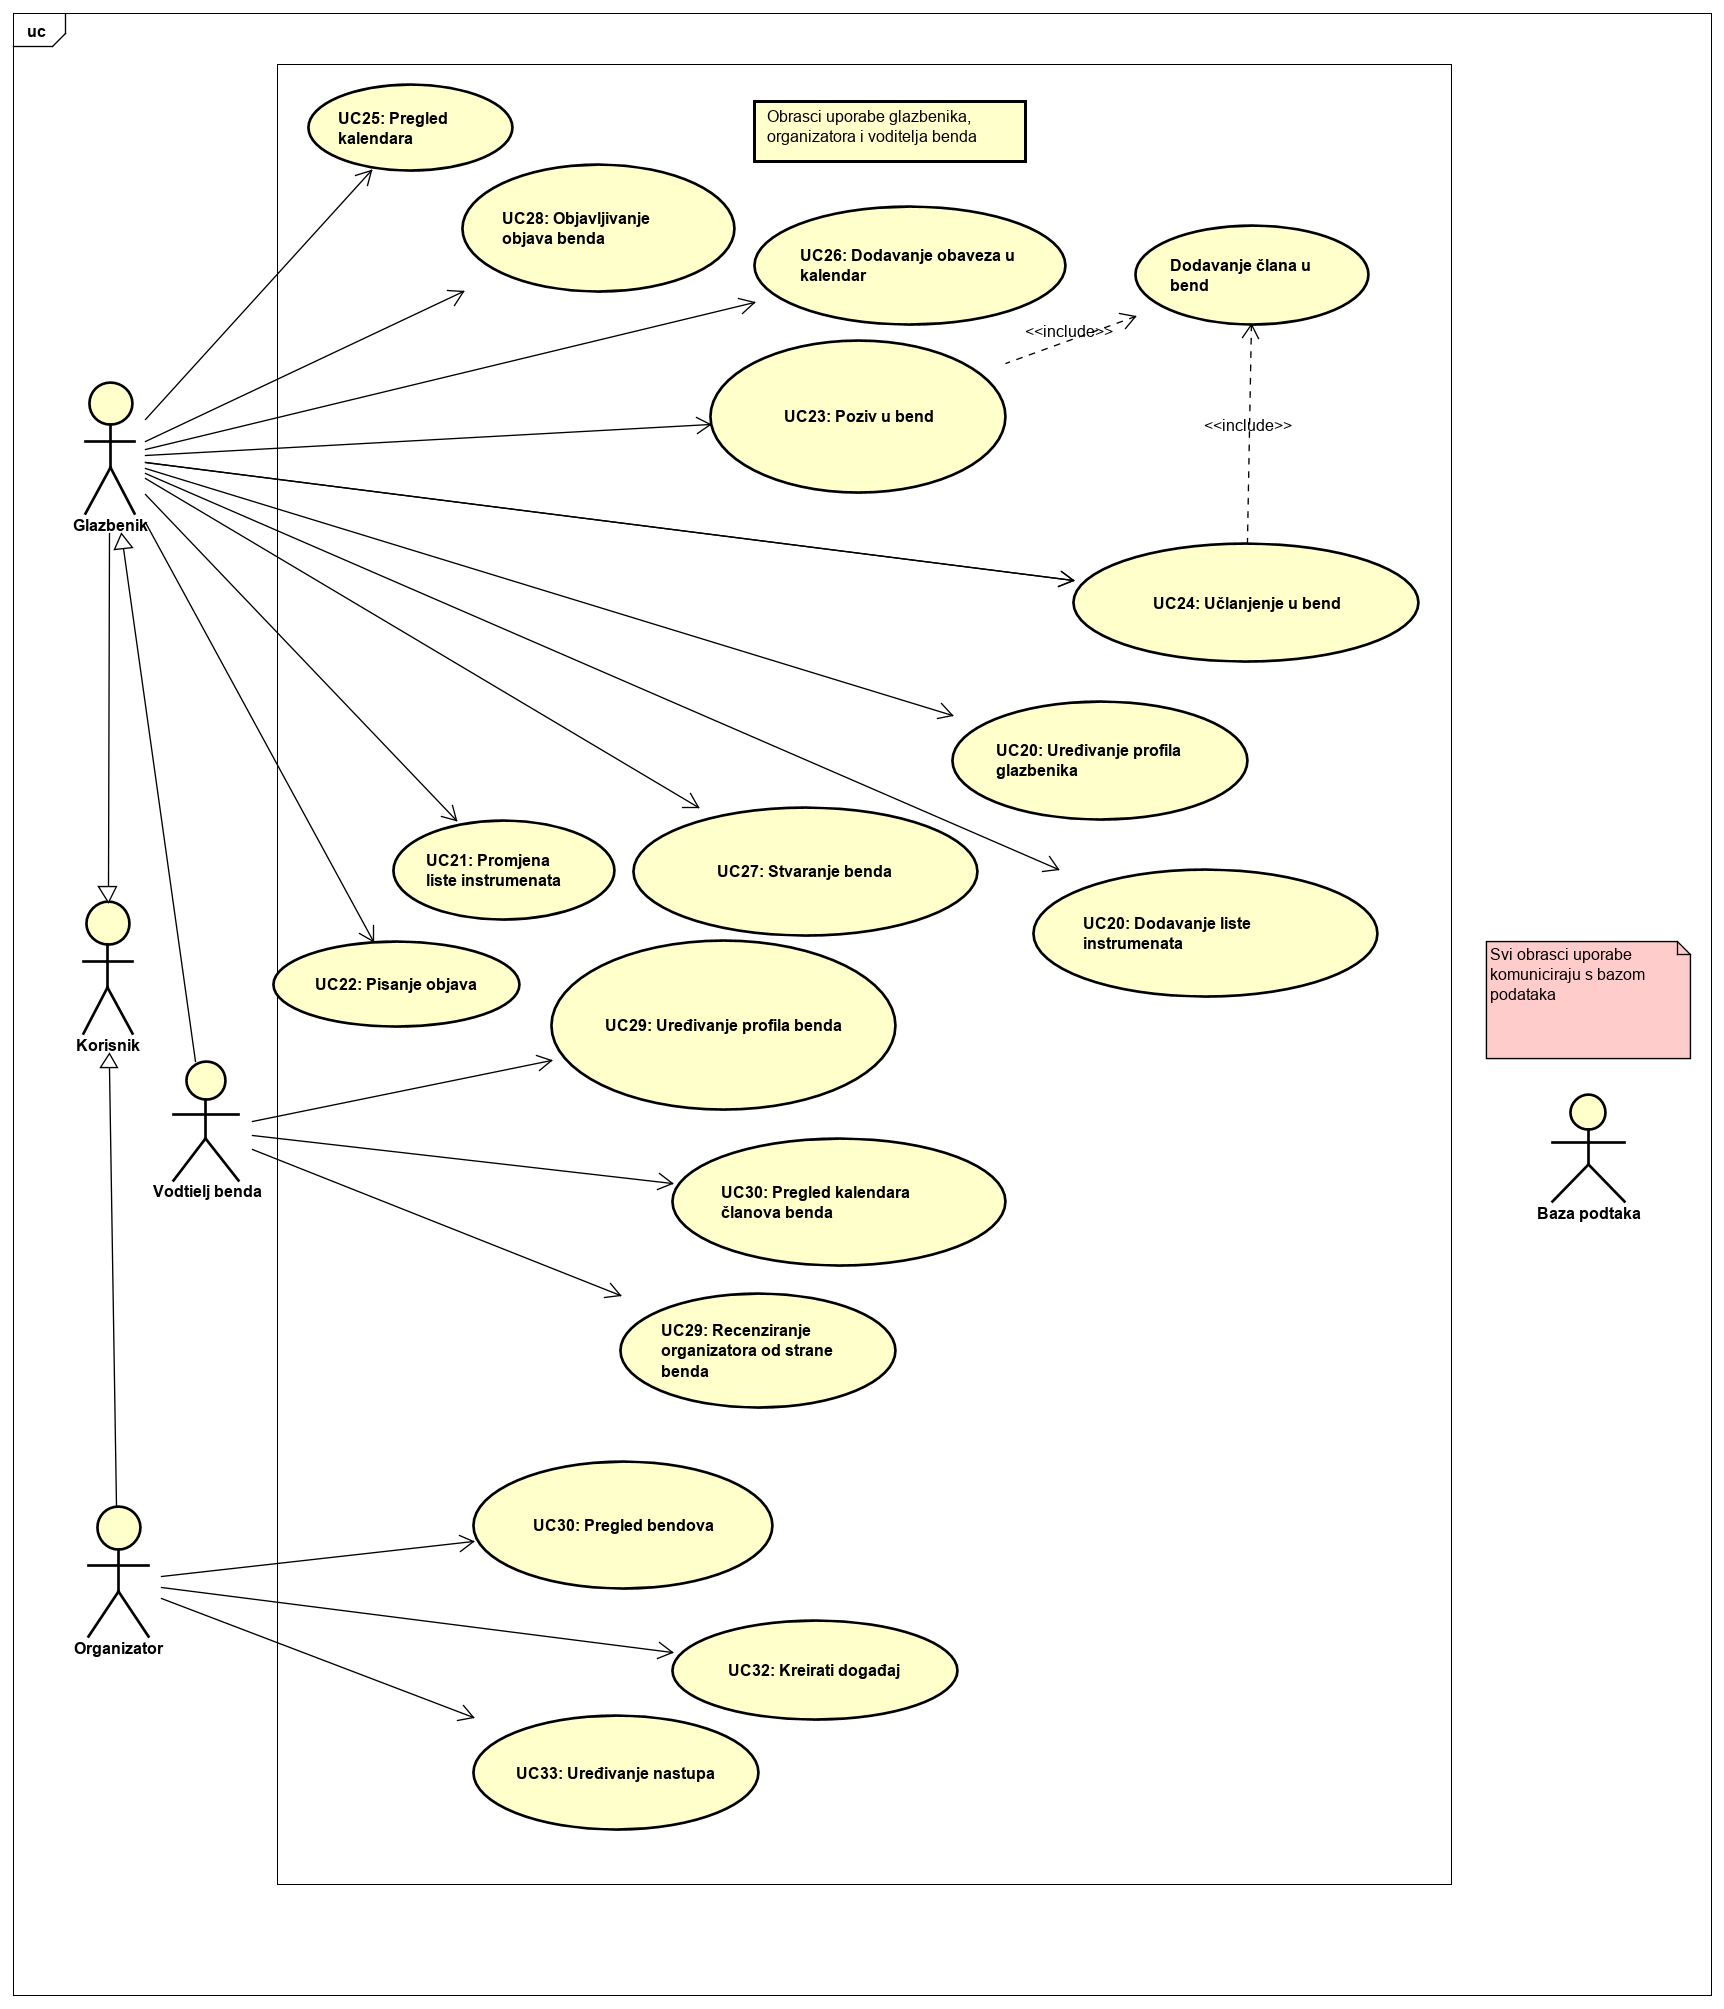
\includegraphics[width=17cm]{slike/glazbenik_organizator.PNG}
				\end{center}
				\caption{Obrasci uporabe za korisnika i organizatora}
				\label{fig:ou1}
			\end{figure}
		
		\begin{figure}[H]
		\begin{center}
			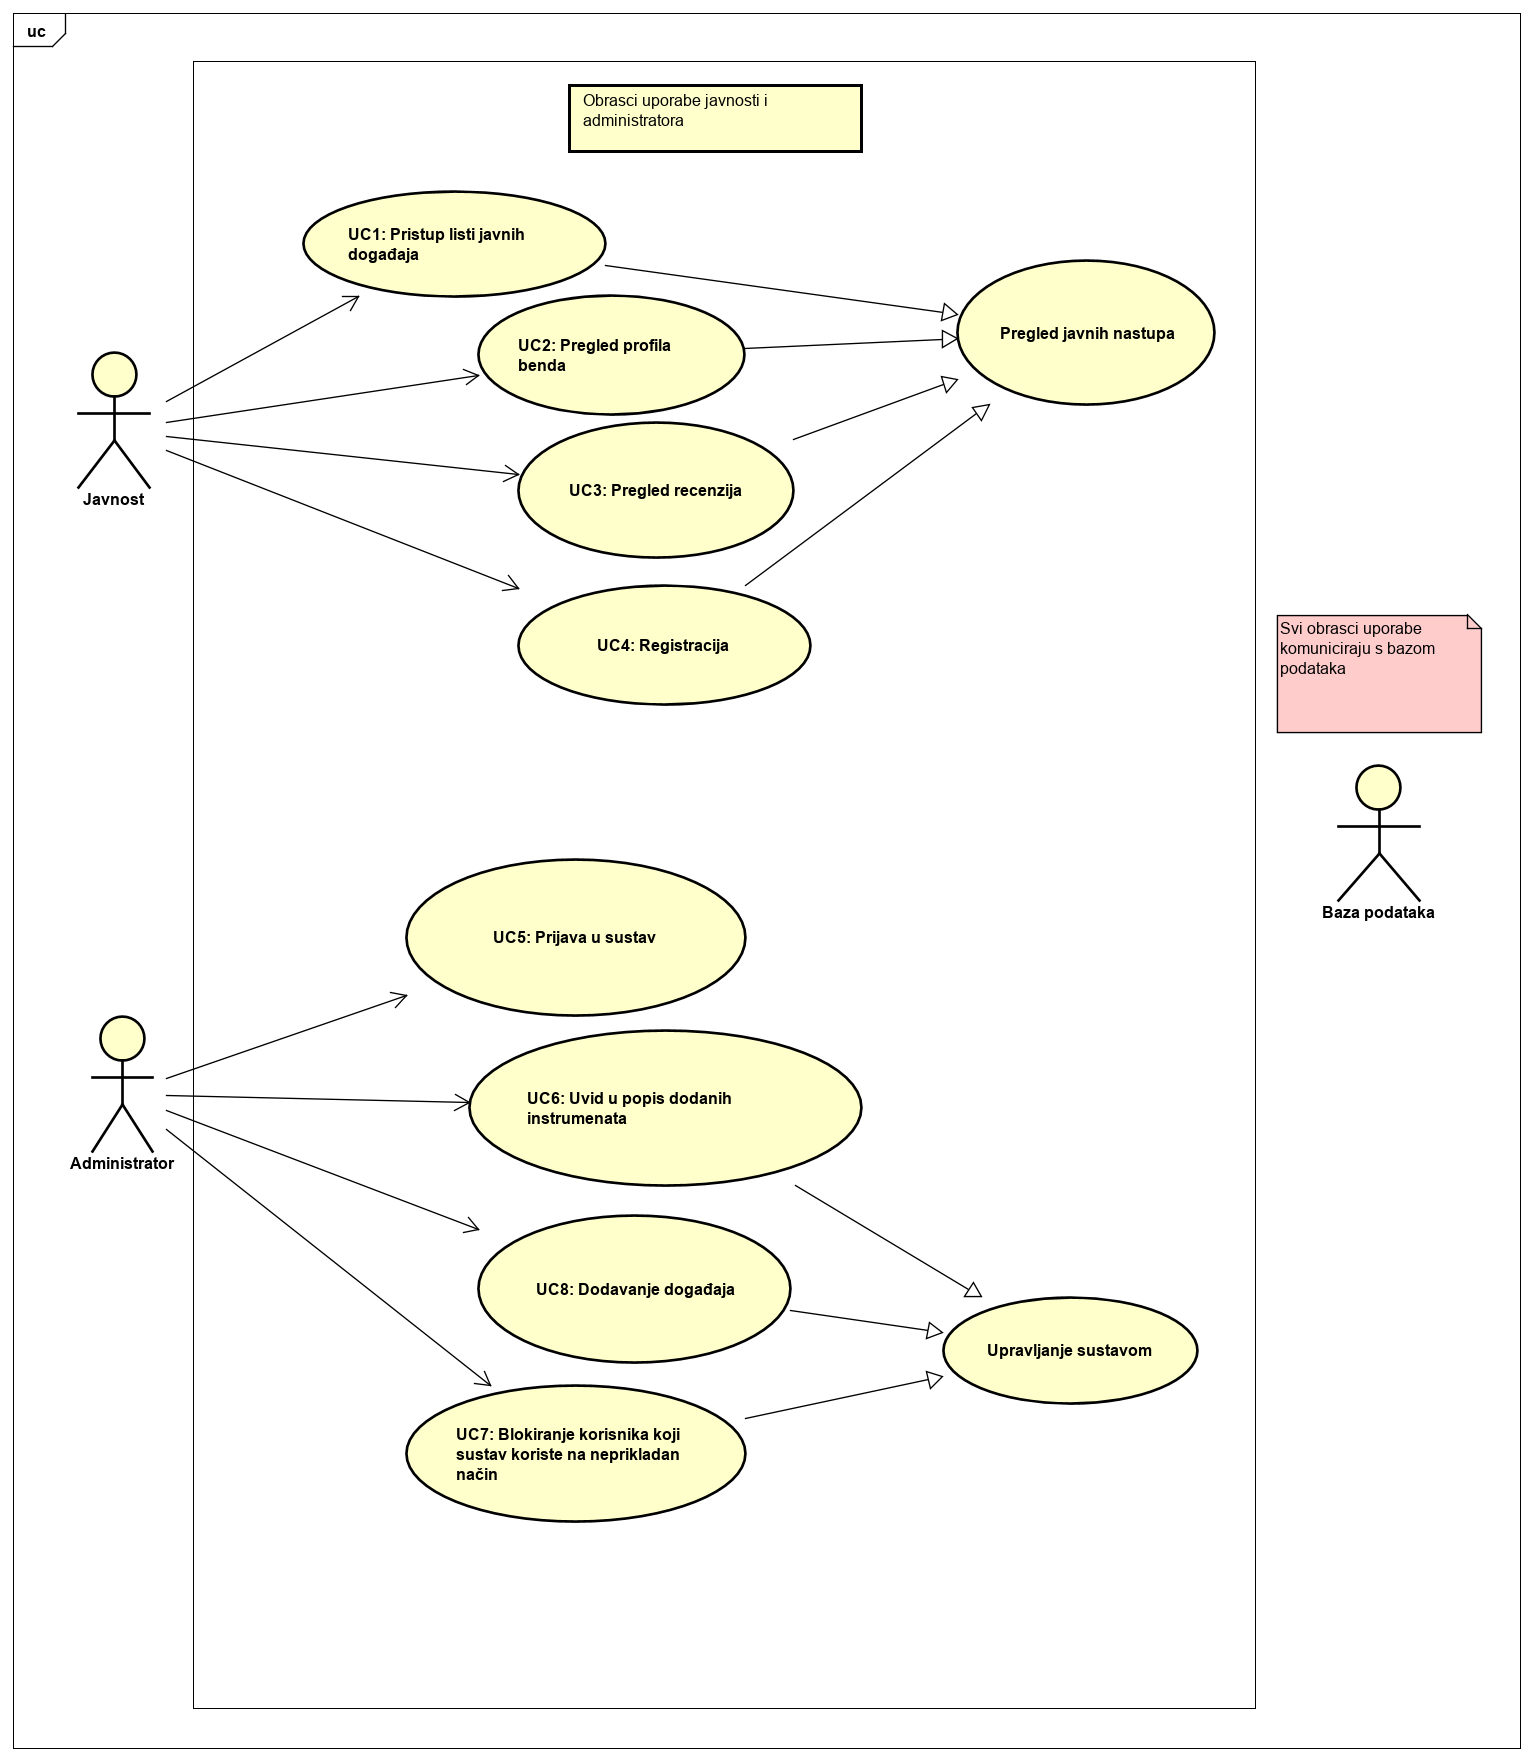
\includegraphics[width=17cm]{slike/javnost_admin2.PNG}
		\end{center}
		\caption{Obrasci uporabe za javnost i administratora}
		\label{fig:ou2}
	\end{figure}

		\begin{figure}[H]
			\begin{center}
				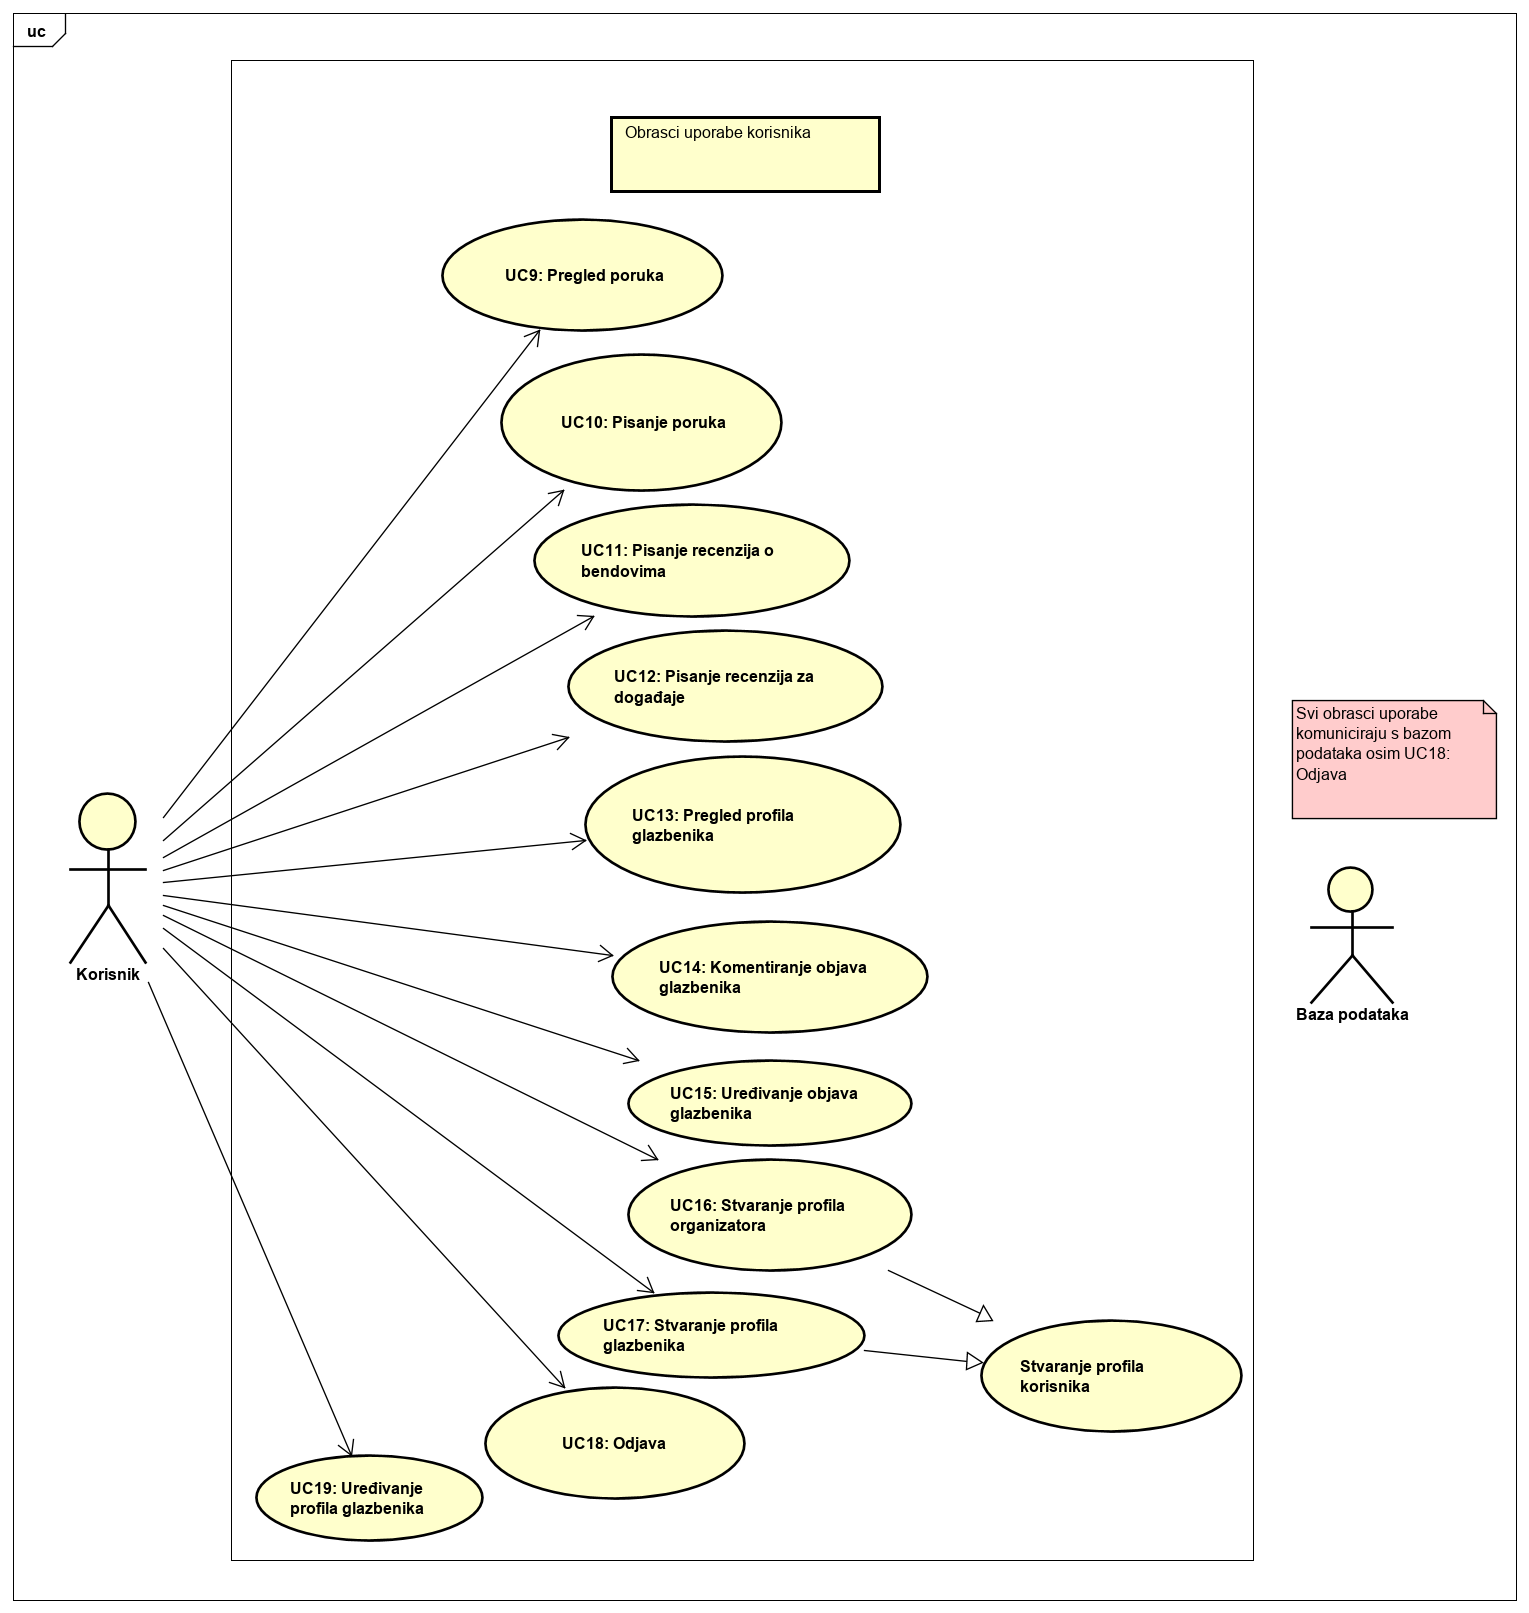
\includegraphics[width=17cm]{slike/korisnik.PNG}
			\end{center}
			\caption{Obrasci uporabe za korisnika}
			\label{fig:ou3}
		\end{figure}
				
				
			\subsection{Sekvencijski dijagrami}
				
				\textbf{Obrazac uporabe UC4 - Registracija}
				\newline
				Javnost (neregistrirani korisnik) odabire opciju za registraciju na što mu aplikacija odgovara prikazom polja za ispunjavanje (korisničko ime, email i lozinka). Dok unos podataka nije ispravan, korisnik unosi podatke te aplikacija dohvaća korisnike iz baze nakon čega provjerava postoji li korisnik istog korisničkog imena ili emaila. Vrši se provjera ispravnosti podataka te ukoliko su podatci valjani, unose se u bazu. Nakon unosa podataka u bazu, korisniku se šalje obavijest o uspješnoj registraciji. 
				
				\begin{figure}[H]
					\begin{center}
						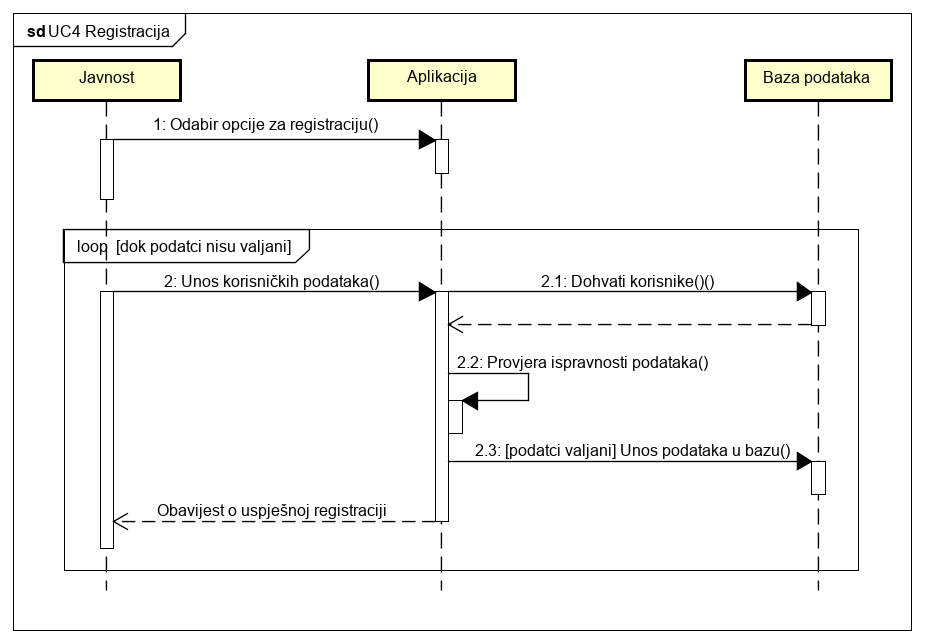
\includegraphics[width=15cm]{slike/UC4.PNG}
					\end{center}
					\caption{Sekvencijski dijagram za UC4}
					\label{fig:uc4}
				\end{figure}
			
				\textbf{Obrazac uporabe UC10 - Pisanje poruke}
				\newline
				Korisnik odabire "Poruke" nakon čega se iz baze dohvaćaju postojeće poruke korisnika. Korisnik može ili napraviti novi razgovor, ili odabrati postojeći. Ukoliko želi napraviti novi razgovor, odabire opciju "Nova poruka" te mu se prikaže prazna poruka. Nakon toga, odabire korisnika kojemu želi napisati poruku, a taj korisnik se traži u bazi podataka. Ukoliko korisnik želi razgovarati s korisnikom s kojim je već komunicirao, odabire razgovor s tim korisnikom. Aplikacija dohvaća iz baze podataka prošle poruke s odabranim korisnikom. U oba opisana slučaja, korisnik piše željenu poruku te ju šalje nakon čega se poruka sprema u bazu.
			
				\begin{figure}[H]
					\begin{center}
						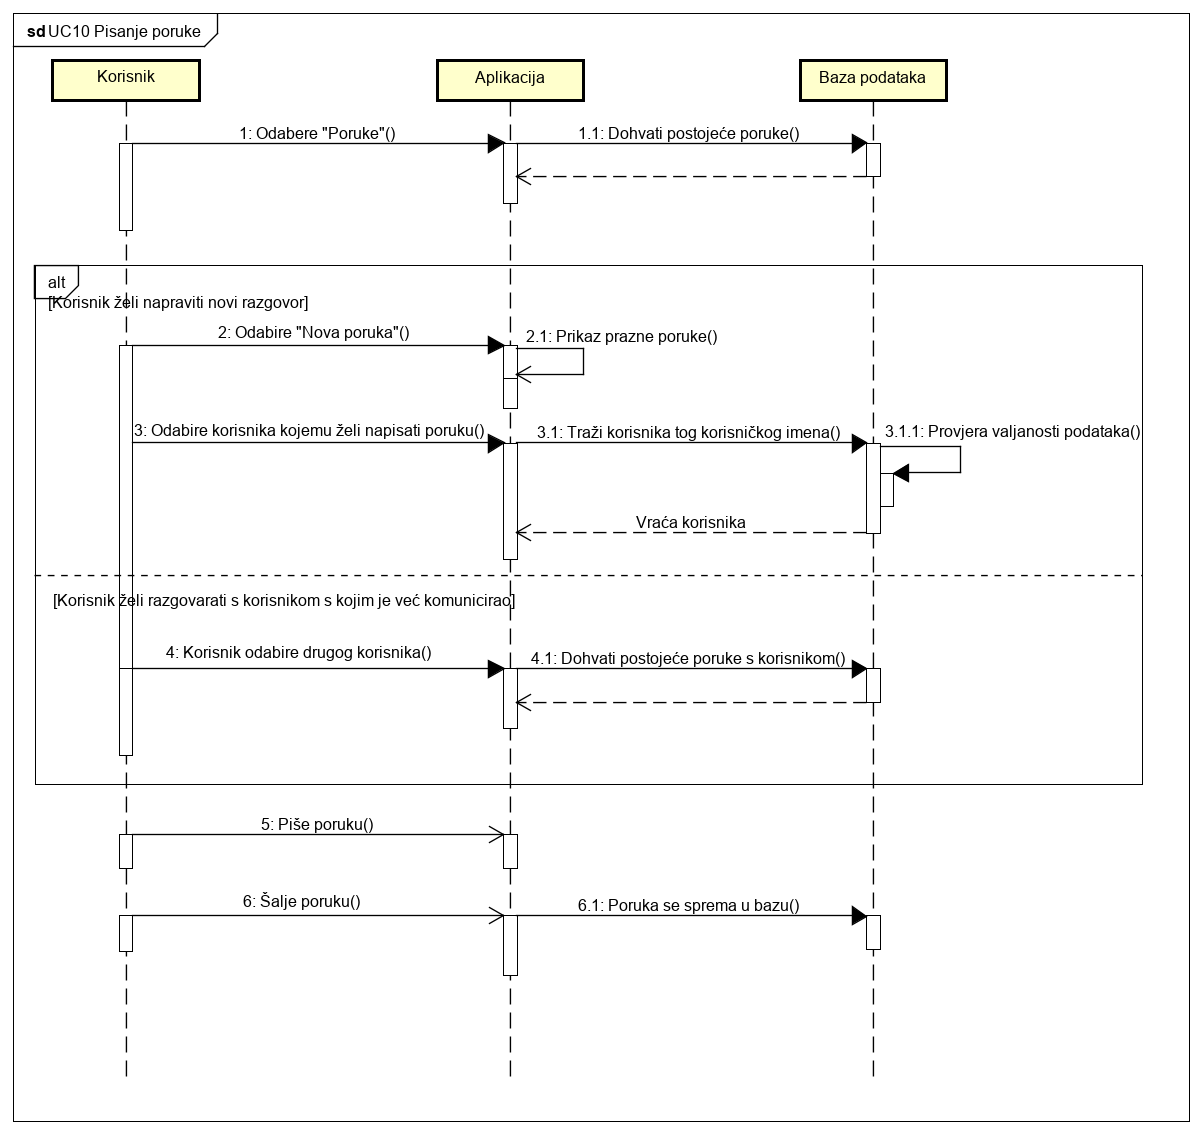
\includegraphics[width=15cm]{slike/UC10.PNG}
					\end{center}
					\caption{Sekvencijski dijagram za UC10}
					\label{fig:uc10}
				\end{figure}
				
				\eject
				 \textbf{Obrazac uporabe UC15 - Uređivanje profila korisnika}
			\newline
			{Prijavljeni korisnik ide na stranicu svog profila.
			Korisnik potom bira opciju izmjene podataka na svom profilu, nakon čega slijedi proces autentikacije korisnika. Ukoliko je autentikacija prošla, omogućene su izmjene podataka korisniku. Korisnik po želji mijenja podatke nakon čega odabire opciju "Izmijeni". Promijenjeni podatci se zapisuju u bazu, a korisniku se prikazuje izmijenjena stranica profila.}\\
				
				
				\begin{figure}[H]
					\begin{center}
						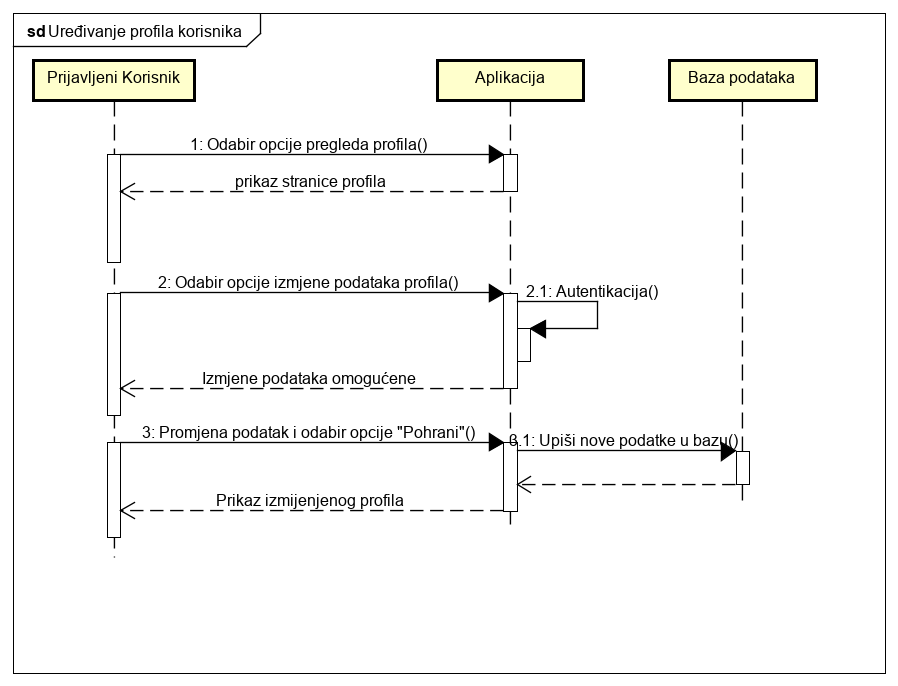
\includegraphics[width=15cm]{slike/uc15_fixed.PNG}
					\end{center}
					\caption{Sekvencijski dijagram za UC15}
					\label{fig:uc15}
				\end{figure}
				
				
				
			\eject
				 \textbf{Obrazac uporabe UC24 - Pregled kalendara}
			\newline
			Prijavljeni korisnik bira opciju prikaži kalendar, nakon čega aplikacija uzima iz baze podataka sve događaje koji su relevantni za korisnika (one na kojima je bio/će biti ili je svirao/će svirati). Aplikacija puni kalendar tim događajima i prikazuje ih korisniku.\\
			
			\begin{figure}[H]
				\begin{center}
					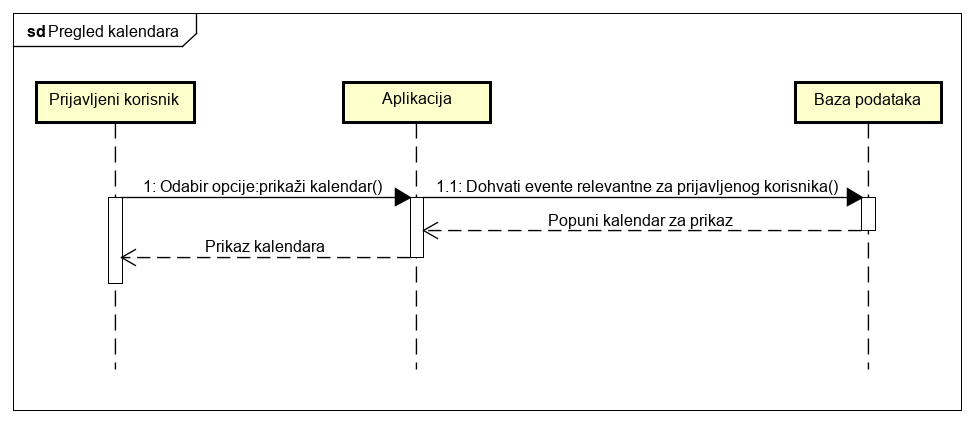
\includegraphics[width=15cm]{slike/uc25.PNG}
				\end{center}
				\caption{Sekvencijski dijagram za UC24}
				\label{fig:uc25}
			\end{figure}
	
		\section{Ostali zahtjevi}
			 \begin{itemize}
			 	\item  Sustav treba omogućiti rad više korisnika u isto vrijeme
			 	\item  Neispravno korištenje sučelja ne smije na bilo koji način promijeniti ili obustaviti rad sustava
			 	\item  Sustav mora biti jednostavan za uporabu, tj. mora biti intuitivan
			 	\item Aplikacija mora podržavati hrvatske dijakritičke znakove
			 	\item  Sustav mora biti u stanju brzo obraditi dobivene podatke kako korisnik ne bi dugo čekao promjenu
			 	\item  Sustav treba biti implementiran kao web aplikacija, s tim da bi joj većina korisnika pristupala preko mobilnih uređaja
			 	\item Web aplikacija treba biti implementirana koristeći objektno-orijentirane jezike
			 	\item  Treba osigurati sigurnost aplikacije, tj. lozinke moraju biti enkriptirane te mora biti osigurana sigurnost veze između korisnika aplikacije i baze podataka 
			 \end{itemize}